\documentclass[a4paper,11pt]{jsarticle}

% 数式
\usepackage{amsmath,amsfonts}
\usepackage{bm}
% 画像
\usepackage[dvipdfmx]{graphicx}
% bibTeX
\usepackage[backend = biber,style =apa, sorting =none,]{biblatex}

% 参考文献ファイルのリスト
% \addbibresource{references.bib}

% 等式番号を章ごとに割り振る
\makeatletter
\@addtoreset{equation}{section}
\def\theequation{\thesection.\arabic{equation}}
\makeatother

% ハイパーリンク
\usepackage[dvipdfmx]{hyperref}
\usepackage{pxjahyper}

% listings(ソースコード)
\usepackage{listings}
\usepackage{color}

\definecolor{dkgreen}{rgb}{0,0.6,0}
\definecolor{gray}{rgb}{0.5,0.5,0.5}
\definecolor{mauve}{rgb}{0.58,0,0.82}

\lstset{
language=Python,
basicstyle=\small\sffamily,
numbers=left,
numberstyle=\tiny\color{gray},
keywordstyle=\color{blue},
commentstyle=\color{dkgreen},
stringstyle=\color{mauve},
frame=single,
columns=fullflexible,
showspaces=false,
showstringspaces=false,
tabsize=3
}
\renewcommand{\lstlistingname}{}

\begin{document}

\title{計算機科学実験4 音声 レポート3}
\author{
  京都大学工学部情報学科\\
  計算機科学コース3回生\\
  学生番号: 1029-33-1415\\
  氏名: 安済翔真
}
\date{\today}
\maketitle

\tableofcontents
\newpage

\section{機能・プログラム説明}
\subsection{音量の表示}
マイクからの入力の音量を表示できるようにした。
コード\ref{code:volume}は音量を表示するためのプログラムである。
本課題ではストリーム処理を行うため、データ列の最後に現在のフレームの音量を追加している。

\begin{lstlisting}[caption=音量の表示,label=code:volume]
vol = 20 * np.log10(np.mean(x_current_frame ** 2) + EPSILON)
volume_data = np.roll(volume_data, -1)
volume_data[-1] = vol
\end{lstlisting}

\subsection{スペクトログラムの表示}
マイクからの音声のスペクトログラムを表示できるようにした。
コード\ref{code:spectrogram}はスペクトログラムを表示するためのプログラムである。
音量が一定以下のときはスペクトログラムを表示しないようにしている。

\begin{lstlisting}[caption=スペクトログラムの表示,label=code:spectrogram]
fft_spec = np.fft.rfft(x_stacked_data * hamming_window)
fft_log_abs_spec = np.log10(np.abs(fft_spec) + EPSILON)[:-1]

spectrogram_data = np.roll(spectrogram_data, -1, axis=1)
spectrogram_data[:, -1] = fft_log_abs_spec
if vol < VOLUME_THRESHOLD:
  spectrogram_data[:, -1] = np.array(fft_log_abs_spec) * np.nan
\end{lstlisting}

\subsection{音程の表示}
マイクからの音声の音程を表示できるようにした。
コード\ref{code:note}は音程を表示するためのプログラムである。
音量が一定以下のときは音程を表示しないようにしている。

\begin{lstlisting}[caption=音程の表示,label=code:note]
melody = shs(fft_log_abs_spec, SAMPLING_RATE, FRAME_SIZE)
  melody_data = np.roll(melody_data, -1)
  if vol < VOLUME_THRESHOLD:
    melody = np.nan # 話していないときは音程を0にする
  melody_data[-1] = melody - NOTES[0]
\end{lstlisting}


\subsection{音楽の再生・再生時間の表示}
予め指定した音楽を再生できるようにした。
コード\ref{code:music}は音楽を再生するためのプログラムである。
音楽の再生にはpyaudioを用いている。

\begin{lstlisting}[caption=音楽の再生,label=code:music]
p_play = pyaudio.PyAudio()
stream_play = p_play.open(
  format = p.get_format_from_width(audio_data.sample_width),	
  channels = audio_data.channels,								
  rate = audio_data.frame_rate,								
  output = True												
)
for chunk in make_chunks(audio_data, size_frame_music):
  stream_play.write(chunk._data)
\end{lstlisting}

\subsection{終了ボタン}
アプリを終了できるボタンを配置した。
コード\ref{code:quit}は終了ボタンを配置するためのプログラムである。
終了ボタンを押すと画面が閉じるようになっている。

\begin{lstlisting}[caption=終了ボタン,label=code:quit]
button = tkinter.Button(master=root, text="終了", command=_quit, font=("", 30))
button.pack()
\end{lstlisting}

\section{実行例とテスト}
\subsection{音量の表示}
アプリを開くと図\ref{fig:volume}のように音量が表示される。
音量は右側の軸で表示されている。

\begin{figure}[h]
\centering
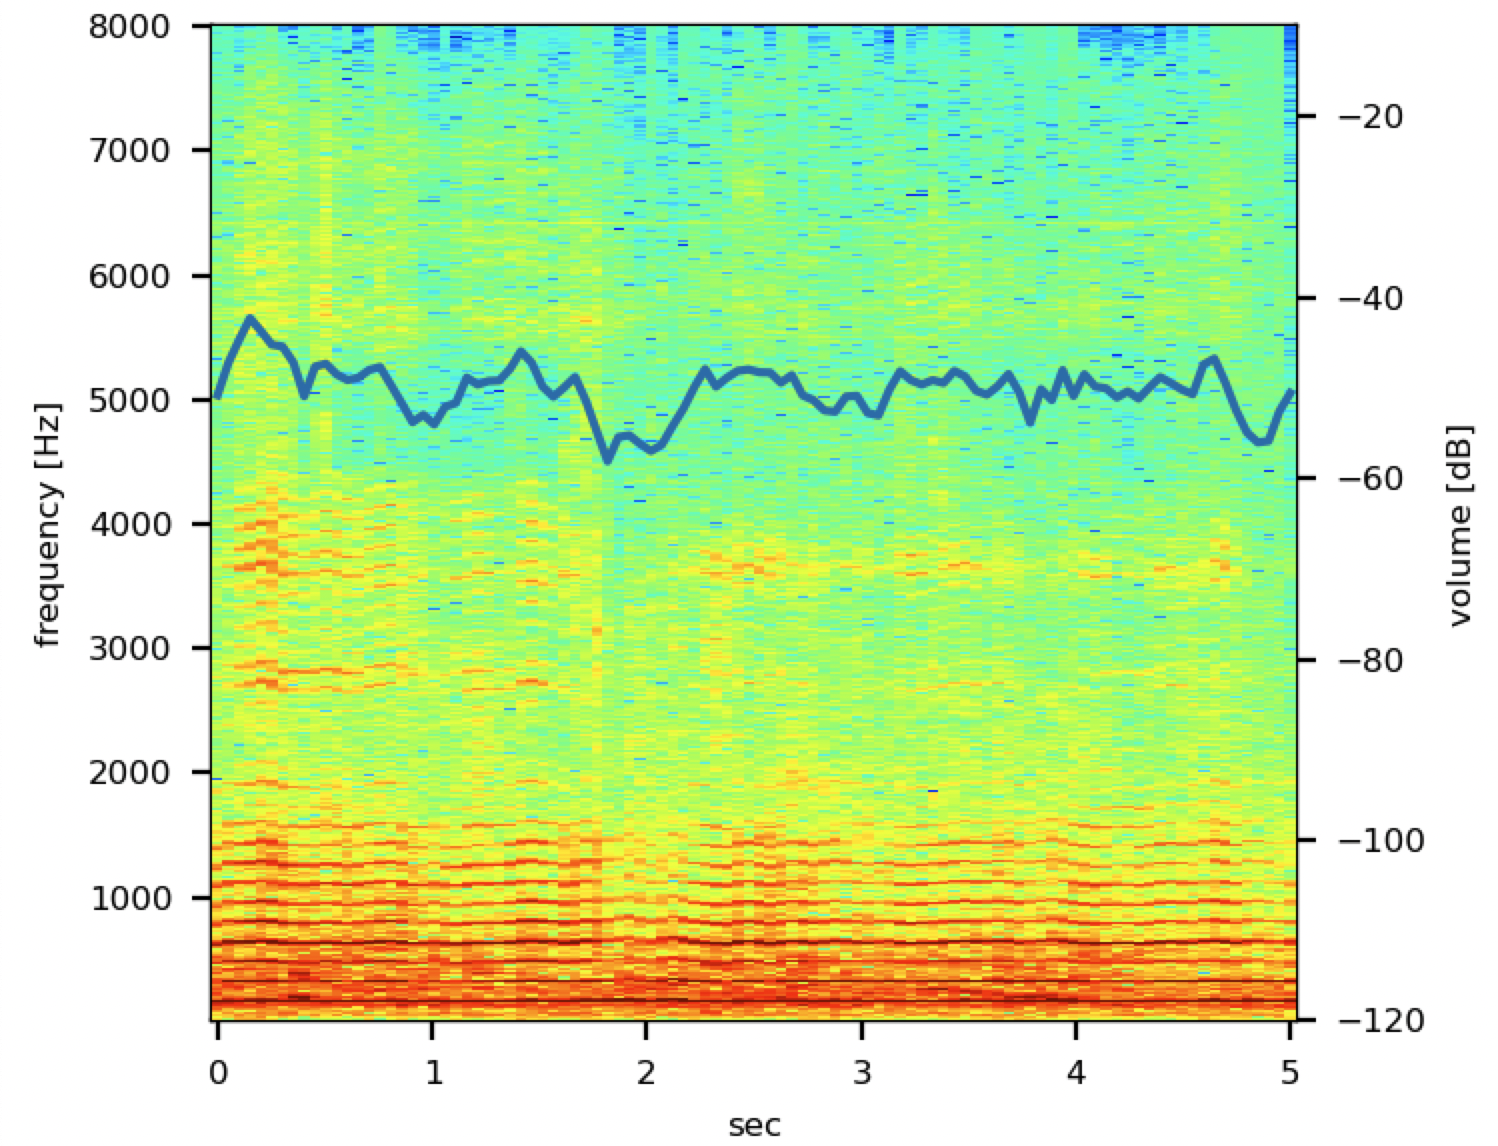
\includegraphics[keepaspectratio, width=13cm]
{./images/work3_spec_volume.png}
\caption{音量の表示}
\label{fig:volume}
\end{figure}

\subsection{スペクトログラムの表示}
アプリと開くと図\ref{fig:spec}のようにスペクトログラムが表示される。
声を出していない区間ではスペクトログラムが表示されないことを確認した。

\begin{figure}[h]
\centering
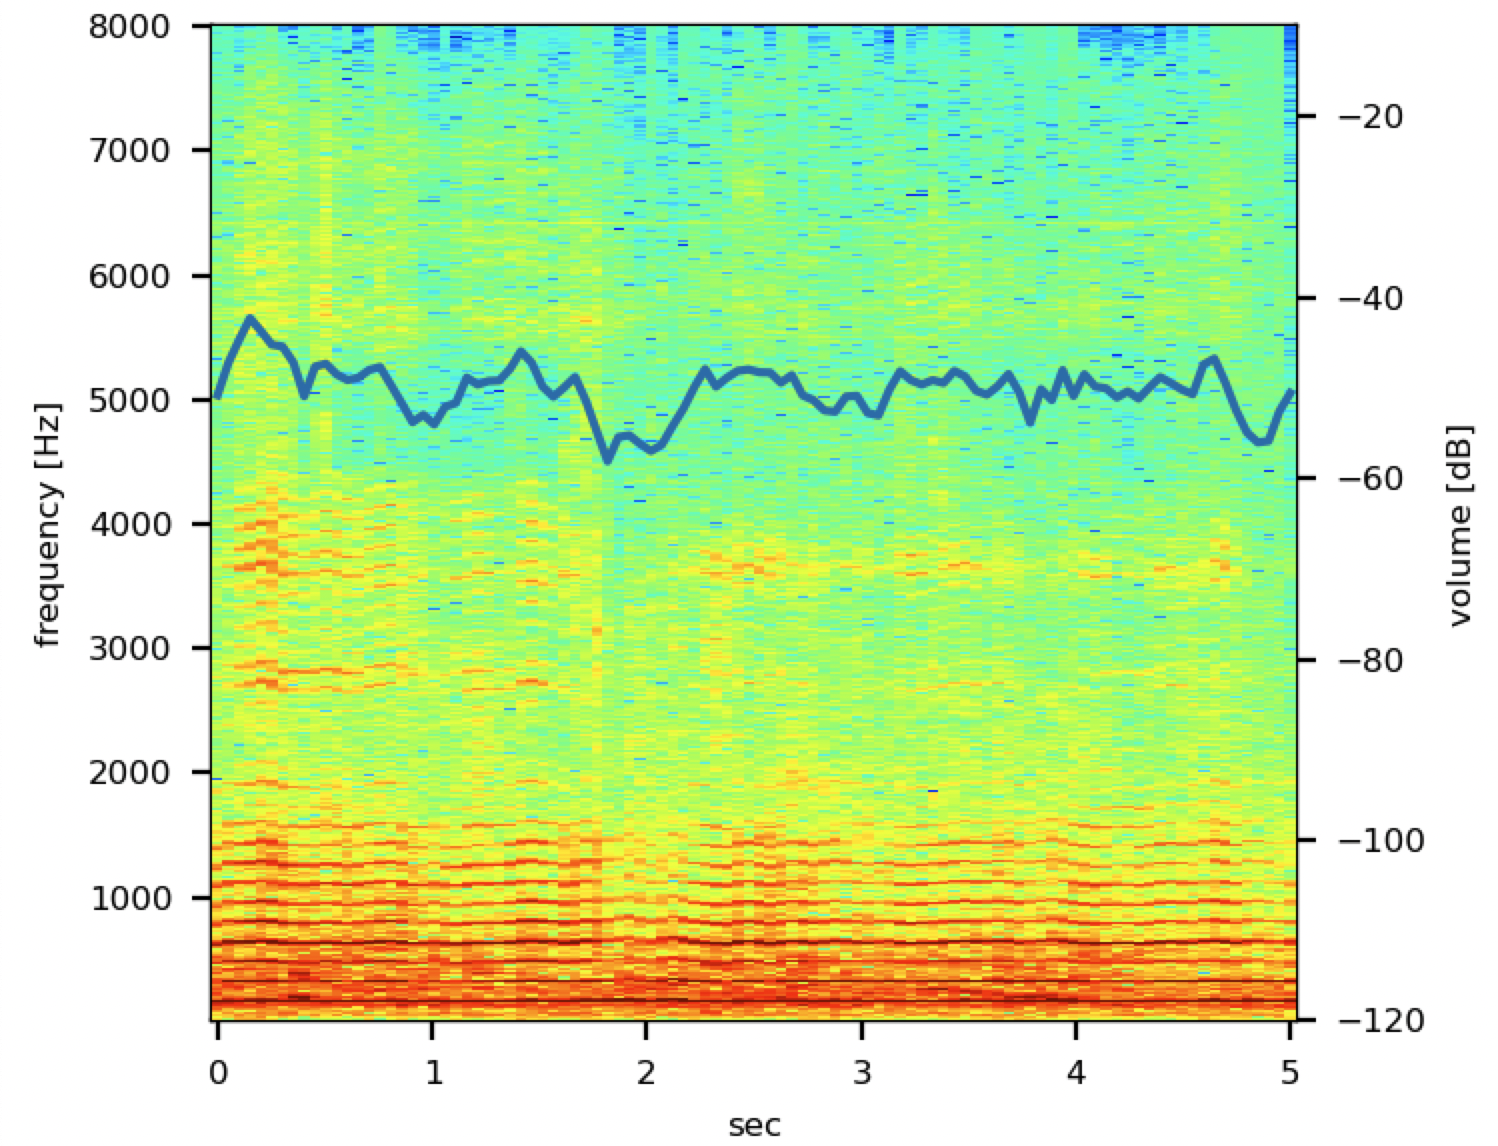
\includegraphics[keepaspectratio, width=13cm]
{./images/work3_spec_volume.png}
\caption{スペクトログラムの表示}
\label{fig:spec}
\end{figure}


\subsection{音程の表示}
アプリを開くと図\ref{fig:note}のように音程が表示される。
声を出していない区間では音程が表示されないことを確認した。

\begin{figure}[h]
\centering
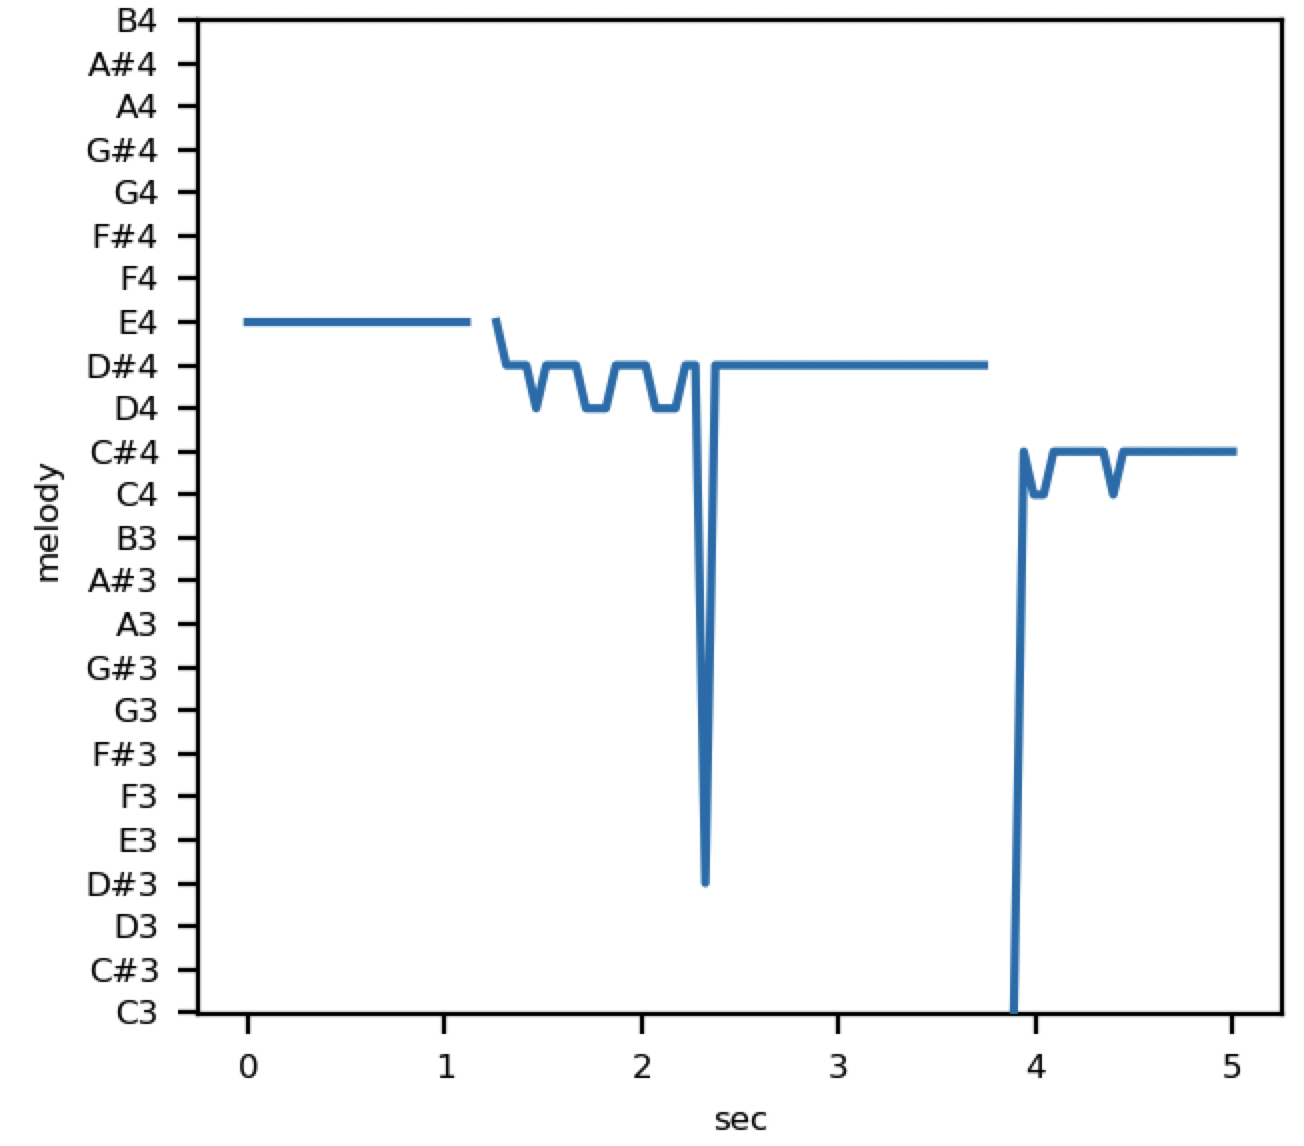
\includegraphics[keepaspectratio, width=13cm]
{./images/work3_melody.png}
\caption{音程の表示}
\label{fig:note}
\end{figure}

\subsection{音楽の再生・再生時間の表示}
アプリを開くと音楽が再生される。また、図\ref{fig:music}のように再生時間が表示されることを確認した。

\begin{figure}[h]
\centering
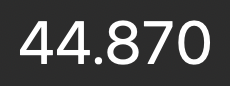
\includegraphics[keepaspectratio, width=13cm]
{./images/work3_play_time.png}
\caption{音楽の再生・再生時間の表示}
\label{fig:music}
\end{figure}


\subsection{終了ボタン}
アプリを開くと終了ボタンが表示される。
終了ボタンを押すとアプリが終了することを確認した。

\begin{figure}[h]
\centering
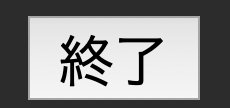
\includegraphics[keepaspectratio, width=13cm]
{./images/work3_quit.png}
\caption{終了ボタン}
\label{fig:quit}
\end{figure}

\section{工夫点}
\subsection{音量の表示}
マイクからの入力音声の音量を表示できるようにした。
これにより、音の大きさを可視化し、音声の強弱を把握できるようになった。

\subsection{音程の軸の表示}
音程の軸を、ノート番号ではなく、音程の名前で表示できるようにした。(図\ref{fig:note})
これにより、音程の把握が容易になった。

\subsection{再生時間の表示}
音楽の再生時間を表示できるようにした。これにより、歌い始めてからの経過時間を把握できるようになった。

\section{考察}
今回の課題では、入力音声のストリーム処理を行った。入ってくる入力を逐次処理するのは、状態の
管理などが難しかったが良い経験になった。

% \printbibliography[title=参考文献]

\end{document}
